\documentclass[twocolumn]{article}
\usepackage{amsmath}
\usepackage{xcolor}
\usepackage{graphicx}
\usepackage{caption}
\usepackage{fancyhdr}
\usepackage{geometry}
\usepackage{enumitem}
\usepackage{array}
\usepackage{hyperref}
\geometry{margin=0.7in}
\pagestyle{empty}

\begin{document}

\begin{figure}[t]
    
\includegraphics[width=\linewidth]{img3.png} % Make sure image file is in same directory
    \textbf{Name: K.Saisusmitha} \\
    \textbf{Batch: 2} \\
    \textbf{ID: cometfwc018} \\
    \textbf{Date: 9th July 2025}
\end{figure}

\begin{center}
    {\LARGE \textbf{\textcolor{blue}{GATE Question Paper 2010, EC Question Number 11}}}
\end{center}

\vspace{1em}
\begin{figure}[h]
    \centering
    \includegraphics[width=\linewidth]{ec2010 11.png}
\end{figure}

\section*{\textcolor{blue}{Question Analysis}}
\textbf{Given:} Column A shows standard logic gates; Column B shows equivalent forms.  
\textbf{Task:} Match logic gate in Column A with its equivalent in Column B.

\section*{\textcolor{blue}{Step-by-Step Matching}}

\begin{enumerate}[label=\textbf{Step \arabic*:}]
    \item \textbf{P (Column A)} – NOR gate (OR + NOT).  
    Matched with Column B Option 4.
    
    \item \textbf{Q (Column A)} – NAND gate (AND + NOT).  
    Matched with Column B Option 2.

    \item \textbf{R (Column A)} – XOR gate.  
    Matched with Column B Option 3.

    \item \textbf{S (Column A)} – AND gate.  
    Matched with Column B Option 1.
\end{enumerate}

\section*{\textcolor{blue}{Correct Option: (D)}}
\[
\boxed{\text{P-4, Q-2, R-3, S-1}}
\]

\section*{\textcolor{blue}{Truth Table for Basic Gates}}

\begin{table}[h]
\centering
\renewcommand{\arraystretch}{1.3}
\begin{tabular}{|c|c|c|c|c|c|}
\hline
A & B & AND & OR & XOR & NAND \\
\hline
0 & 0 & 0 & 0 & 0 & 1 \\
0 & 1 & 0 & 1 & 1 & 1 \\
1 & 0 & 0 & 1 & 1 & 1 \\
1 & 1 & 1 & 1 & 0 & 0 \\
\hline
\end{tabular}
\caption*{\textbf{Reference Output Table for Logic Gates}}
\end{table}

\section*{\textcolor{blue}{Hardware Implementation}}

\textbf{Goal:} Implement each gate using buttons as inputs and LEDs as outputs for visual testing.

\subsection*{\textcolor{blue}{Hardware Requirements}}

\begin{table}[h]
\centering
\renewcommand{\arraystretch}{1.3}
\begin{tabular}{|c|l|}
\hline
\textbf{S.No} & \textbf{Component} \\
\hline
1 & Raspberry Pi Pico 2 W / Arduino Uno \\
2 & Breadboard \\
3 & Push Buttons (2x) – for inputs A and B \\
4 & LEDs (4x) – for AND, OR, XOR, NAND outputs \\
5 & Resistors (220$\Omega$ for LEDs, 10k$\Omega$ for buttons) \\
6 & Jumper wires \\
7 & Micro USB cable \\
\hline
\end{tabular}
\caption*{\textbf{List of Required Components}}
\end{table}

\subsection*{\textcolor{blue}{GPIO Pin Mapping – Pico 2 W}}

\begin{table}[h]
\centering
\renewcommand{\arraystretch}{1.3}
\begin{tabular}{|c|c|c|}
\hline
\textbf{Component} & \textbf{Pico Pin} & \textbf{Function} \\
\hline
Button A & GP14 & Logic Input A \\
Button B & GP15 & Logic Input B \\
AND LED & GP10 & Output of A·B \\
OR LED & GP11 & Output of A+B \\
XOR LED & GP12 & Output of A$\oplus$B \\
NAND LED & GP13 & Output of $\overline{A\cdot B}$ \\
GND & GND & Common ground \\
3.3V & 3.3V & Pull-up supply \\
\hline
\end{tabular}
\caption*{\textbf{Pico2W GPIO Mapping for Gate Outputs}}
\end{table}

\subsection*{\textcolor{blue}{Arduino Pin Mapping}}

\begin{table}[h]
\centering
\renewcommand{\arraystretch}{1.3}
\begin{tabular}{|c|c|c|}
\hline
\textbf{Component} & \textbf{Arduino Pin} & \textbf{Function} \\
\hline
Button A & D2 & Logic Input A \\
Button B & D3 & Logic Input B \\
AND LED & D4 & Output A·B \\
OR LED & D5 & Output A+B \\
XOR LED & D6 & Output A$\oplus$B \\
NAND LED & D7 & Output $\overline{A\cdot B}$ \\
GND & GND & Common Ground \\
VCC & 5V & Pull-up Supply \\
\hline
\end{tabular}
\caption*{\textbf{Arduino GPIO Mapping for Logic Gate Outputs}}
\end{table}

\subsection*{\textcolor{blue}{Steps to Implement (Pico2W)}}

\begin{enumerate}
    \item Connect Pico to PC via USB while holding BOOTSEL.
    \item Copy MicroPython UF2 file.
    \item Open Thonny IDE → Select Interpreter as Raspberry Pi Pico.
    \item Read GPIO pins for A and B.
    \item Calculate AND, OR, XOR, NAND using logic.
    \item Output results to 4 LEDs.
\end{enumerate}

\subsection*{\textcolor{blue}{Steps to Implement (Arduino)}}

\begin{enumerate}
    \item Connect Arduino Uno via USB.
    \item Open Arduino IDE.
    \item Select Board: Arduino Uno; correct COM Port.
    \item Write and upload code to read inputs A and B.
    \item Calculate logic functions and output to LEDs.
    \item Observe logic gate operations physically.
\end{enumerate}

\section*{\textcolor{blue}{Conclusion}}

\begin{figure}[h]
    \centering
    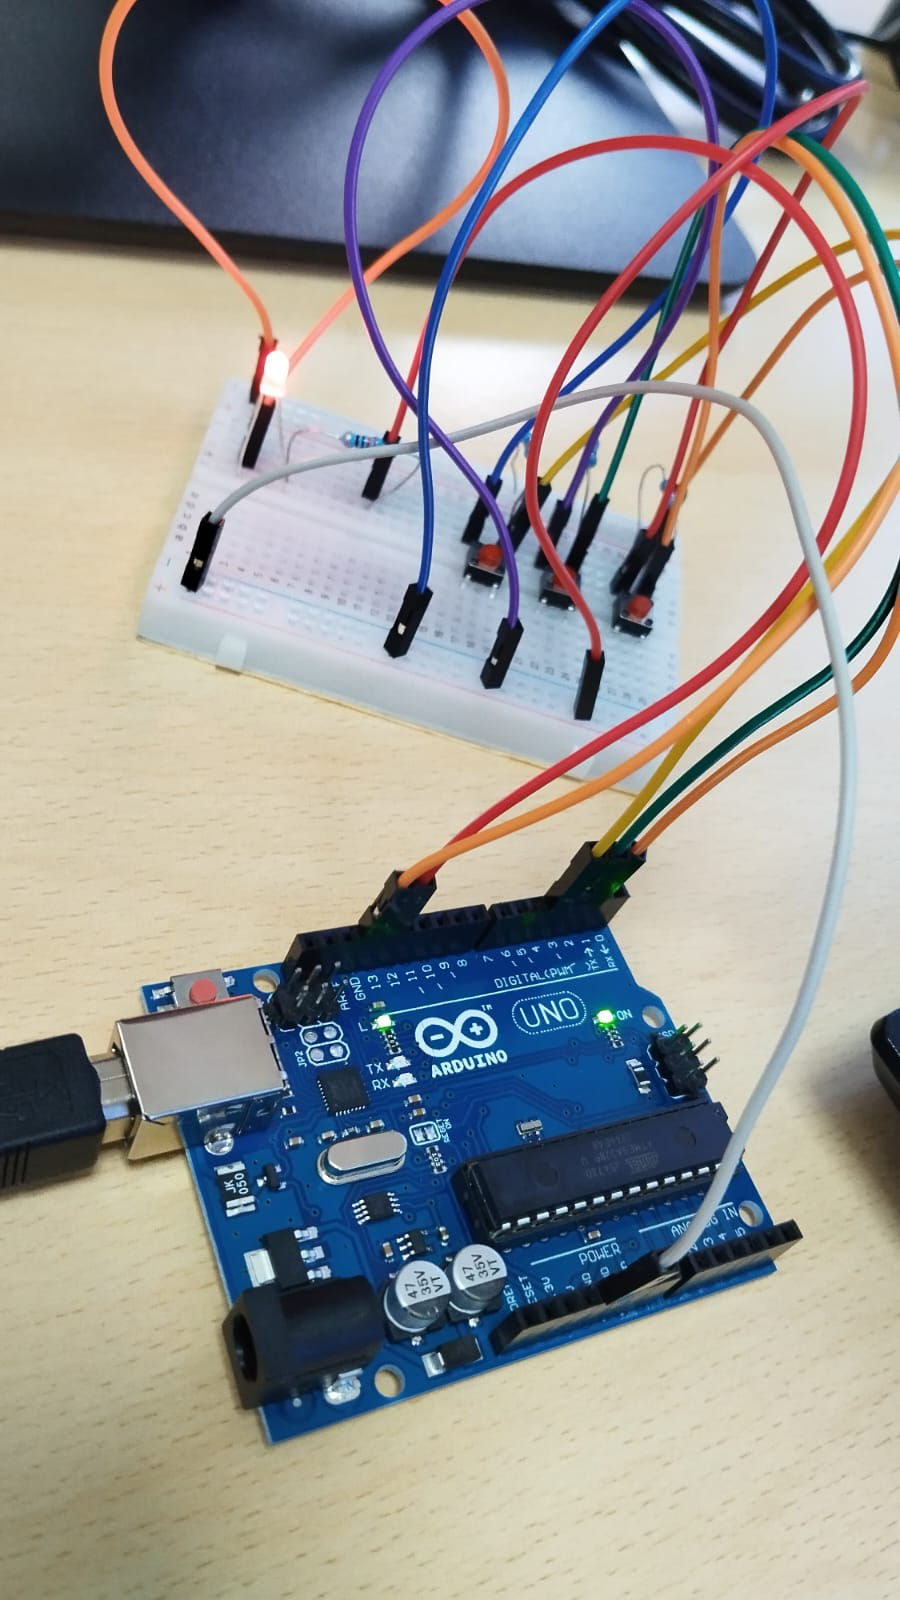
\includegraphics[width=0.95\linewidth]{arm.jpeg}
        \caption*{\textbf{Figure: Hardware Verification Setup (Representative)}}
\end{figure}

\textbf{Summary:}  
Each logic gate was matched to its equivalent using symbol recognition and truth table verification. Hardware implementation using Pico2W or Arduino helps verify gate outputs practically.

\[
\boxed{\text{Correct Answer: Option (D) — P-4, Q-2, R-3, S-1}}
\]

\section*{\textcolor{blue}{Source Code Link}}
The complete hardware simulation and code implementation for this experiment is available at the following GitHub repository:

\textbf{GitHub Repo:} \href{https://github.com/aisusmitha/FWC.git}{github.com/aisusmitha/FWC.git}
\end{document}
